\documentclass[a4paper, 12pt]{scrreprt}
%\documentclass[headsepline,titlepage,twoside,12pt]{report}
\linespread{1.5}
\usepackage[ngerman]{babel}
\usepackage[T1]{fontenc}
\usepackage[utf8]{inputenc}
\usepackage[a4paper,top=4cm,bottom=3cm,left=4cm,right=3cm]{geometry}
\usepackage{amsmath}
\usepackage{amssymb}
\usepackage{color}
\usepackage{graphicx}
\usepackage{soul}
%\usepackage{natbib}
\usepackage{hyperref}
\usepackage{listings}
\usepackage{textcomp}
\usepackage{microtype}
\usepackage{tabularx}
\usepackage{setspace}
\usepackage{booktabs}
\usepackage{float}
\usepackage{mwe}
\usepackage[locale=DE]{siunitx}
%\sisetup{output-decimal-marker = {,}}
\sisetup{decimalsymbol=comma}
\usepackage{todonotes}% Für Anmerkungen
\presetkeys{todonotes}{inline,backgroundcolor=yellow}{}
\usepackage{csquotes}
\MakeOuterQuote{"}
\lstset{frame=tb,
  language=HTML,
  aboveskip=3mm,
  belowskip=3mm,
  showstringspaces=false,
  columns=flexible,
  basicstyle={\small\ttfamily},
  numbers=none,
  numberstyle=\tiny\color{gray},
  keywordstyle=\color{blue},
  commentstyle=\color{teal},
  stringstyle=\color{red},
  breaklines=true,
  breakatwhitespace=true,
  tabsize=3,
  texcl=true,
}

\lstset{
  literate={ö}{{ö}}1
           {ä}{{ä}}1
           {ü}{{ü}}1
}
\title{Besondere Lernleistung}
\author{Gernot Zacharias}
\subtitle{Webanwendung zum Finden eines optimalen Standortes durch Distanzminimierung mithilfe von Online-Kartendiensten}
\begin{document}
%\listoftodos
\maketitle
\cleardoublepage
\tableofcontents
%\chapter* {Inhaltsverzeichnis}
\setcounter{page}{1}
\chapter*{Zusammenfassung}
\addcontentsline{toc}{chapter}{Zusammenfassung}
Durch den aufstrebenden Online-Versandhandel, wie zum Beispiel durch Online-Versandapotheken, entstehen neue Probleme.
Die Versandhändler benötigen Lagerhäuser für ihre Waren und die Fahrtwege vom Lager zum Kunden sollten möglichst minimal gehalten werden, um Zeit und Geld zu sparen.
Durch die Verkürzung der Fahrwege wird auch die Gesundheit und die Natur weniger belastet.
Auch Privatanwender profitieren von kurzen Fahrtwegen.
Dieses Problem lässt sich durch eine Anwendung lösen, die aus der Häufigkeit der angesteuerten Orte eine optimale Position mit möglichst kurzen Fahrwegen bestimmt.
Diese Anwendung kann zum Beispiel auf Basis der Kartendienste von "Google Maps" oder "Open Street Map" realisiert werden.
Dies lies sich am einfachsten durch eine Webanwendung lösen, da diese meistens plattformunabhängig sind.
Somit ist keine Installation von zusätzlicher Software, außer einem aktuellen Webbrowser, nötig.
Des weiteren wurde der freie Kartendienst von \emph{Open Street Map} gewählt, da dieser für nicht kommerzielle Zwecke kostenlos ist.
Auch gibt es für Open Street Map eine größere Auswahl an Nutzerschnittstellen.
Die Anwendung funktioniert sehr gut.%\todo{Fragebogen}
Somit lässt sich auch der Treibstoffverbrauch reduzieren, was dem Geldbeutel und der Umwelt zu Gute kommt.
Es gab auch positives Feedback von anderen Personen, die das Programm getestet haben.
Allerdings bietet die Anwendung auch noch viel Spielraum für individuelle Erweiterungen, Verbesserungen und Änderungen.
\chapter*{Abkürzungsverzeichnis}
\addcontentsline{toc}{chapter}{Abkürzungsverzeichnis}
\begin{tabularx}{\textwidth}{lX}
\toprule
\textrm{Begriff}                &\textrm{Erklärung des Begriffs}\\
\midrule
API		&Application Programming Interface\\
CSS		&Cascading Style Sheets\\
GIS		&Geographic Information System \\
HTML	&Hypertext Markup Language\\
HTTP	&Hypertext Transfer Protocol\\
HTTPS	&Hypertext Transfer Protocol Secure\\
JS		&JavaScript\\
PNG		&Portable Network Graphic\\
%WGS84	&52\\
WWW		&World Wide Web\\

\bottomrule
\end{tabularx}

\chapter{Einleitung}
\section{Gegenstand und Motivation}
\subsection{Gegenstand}
%\todo{Verdoppelung von "sich einen möglichst kurzen Weg". Stört mich nicht aber eventuell den Deutschlehrer.}
%\todo{Ich bin immer vorsichtig mit "viele X" und "immer mehr X" wenn man dazu keine Belege hat.}
Versandhändler suchen eine möglichts kurze Strecke zum Kunden und zur Produktionsstätte.
Auch Normalverbraucher wünschen sich einen möglichst kurzen Weg zu ihrer Arbeit, zum Kindergarten, Arzt, oder zu ihrem (Sport-)Verein und sucht deshalb eine Wohnung von der Er diese Orte auf dem kürzesten Weg erreicht.
\subsection{Problematik}
Durch lange Fahrtwege erhöht sich die Dauer der Fahrt bis zum Ziel und somit der Energieverbrauch sowie die Schadstoffbelastung.
Auch die Kosten erhöhen sich bei langen Fahrten, da der Fahrer und/oder der Treibstoff bezahlt werden muss.
Die Kraftfahrer werden durch längere Strecken stärker belastet und das Risiko für Unfälle aufgrund von Übermüdung steigt.\cite{hoffmann1966belastung}
\section{Motivation}
Durch die Reduktion der Distanz zum Ziel wird der Energieverbrauch und die Zeit verringert, dadurch kann Geld gespart und die Umwelt geschont werden.
Auch wird der Fahrer durch eine geringere Fahrzeit weniger stark belastet.
\section{Problemstellung}
Der Online Versandhandel ist ein zurzeit stark wachsender Sektor der Wirtschaft.\cite{Stepper2016}
Deshalb verwundert es auch nicht das es heutzutage
Es gibt auch Online-Versandapotheken, welche Medikamente an die Haustür liefern.
Dies ist vor allem für bewegungseingeschränkte Personen interessant, da diese sich nun nicht mehr zu nächsten Apotheke bewegen müssen.
Auch ermöglicht es Personen die nicht in der Nähe einer Apotheke wohnen, sich die benötigten Medikamente zu besorgen.
Für die Anbieter dieser Versandapotheken ist es nun interessant herauszufinden, wie man Zeit und Geld beim Versand einsparen kann.
Dazu kann man zum Beispiel die Warenlager dort plazieren, wo die Nachfrage am größten ist.
\section{Zielsetzung}
Das Ziel ist es eine Anwendung zu kreieren, welche aus der Häufigkeit des Ansteuerns von bestimmten Orten, einen Ort bestimmt, von welchem aus die Gesamtdistanz,in Abhängigkeit von der Häufigkeit, zu den gegebenen Orten, möglichst klein ist.
\section{Aufgabenstellung}
Zur Lösung der oben genannten Probleme soll eine Webanwendung erstellt werden, welche eine Karte anzeigt, auf der der Nutzer/-in Standorte auswählt, die er mit einer bestimmten Häufigkeit, die er/sie/es selbst angibt, aufsucht.
%\section{Aufbau der Arbeit}
\newpage
\section{Existierende Lösungen}
\begin{figure}[h]
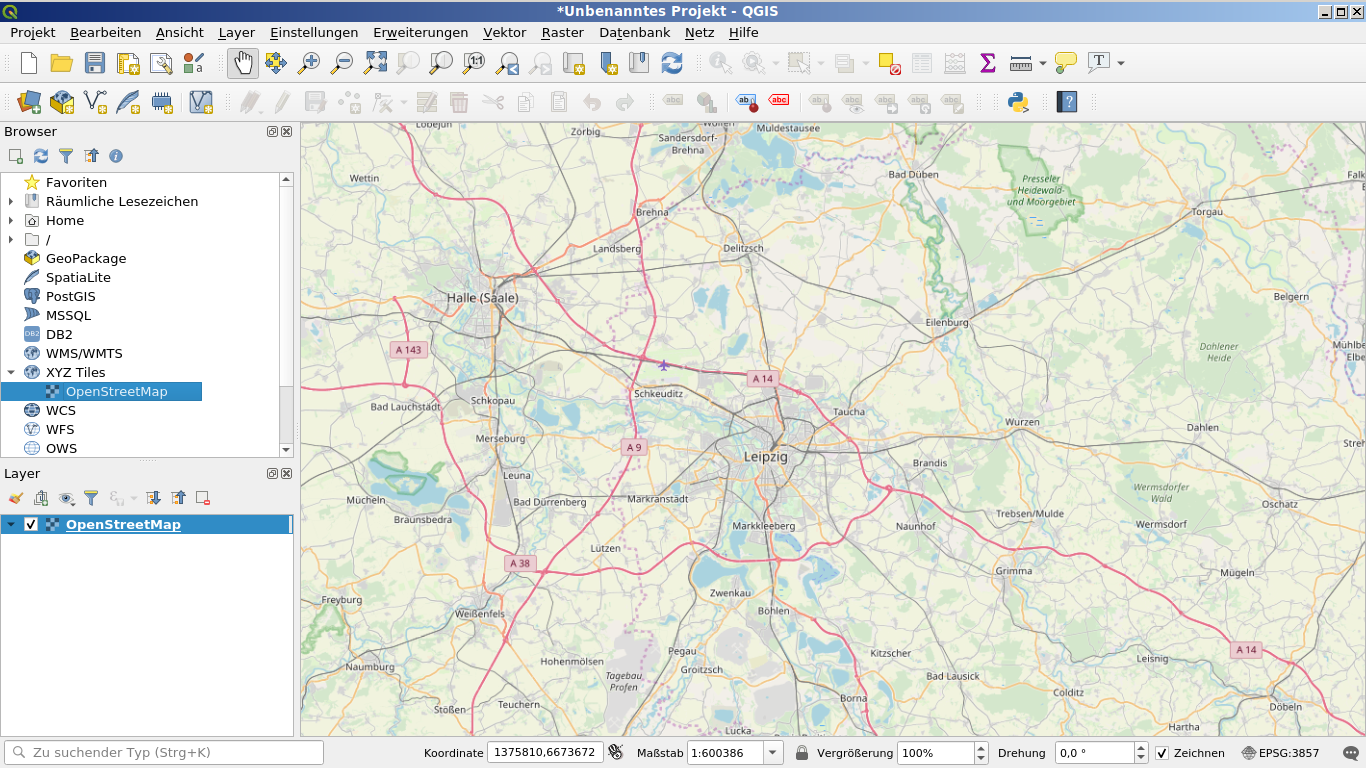
\includegraphics[width=\linewidth]{qgis_oberflaeche.png}
\caption{Screenshot von QGIS 3.10 mit geladener Openstreetmap Karte}
\end{figure}
Die WIGeoGIS\footnote{\url{https://www.wigeogis.com} [02.04.2019 10:58]} Softwareerstellungs- und Handelsgesellschaft m.b.H. bietet verschiedene Services für Kunden aus dem Industriesektor an, unter anderem WebGIS zur Datenanalyse, die über verschiedene Schnittstellen eingebunden werden können, auf digitalen Landkarten. 
Auch bieten sie eine kostenpflichtige Erweiterung des OpenSource Programms QGIS an, um Kunden Daten zur Marktlage oder Bevölkerung zur Verfügung zu stellen.
Das als Opensource verfügbare Programm QGIS ist für Laien recht unübersichtlich und hat einen großen Funktionsumfang.
Bei der Anwendung handelt es sich auch nicht um eine Webanwendung, wodurch der Nutzer zusätzlich Software herunterladen muss.\\

\chapter{Grundlagen}
\section{World Wide Web}
In der heutigen Zeit gewinnt das World Wide Web (WWW) immer mehr an Bedeutung und ist fast schon nicht mehr wegzudenken.
Das World Wide Web ist der Teil des Internets, in dem die Daten mithilfe des HTTP/HTTPS -Protokolls ausgetauscht werden. Dabei sendet ein Computer(Server), auf dem die entsprechenden Daten gespeichert sind, auf Anfrage(Request) durch einen anderen Computer(Client), diesem diese Daten schickt.
Das WWW umfasst also fast alle öffentlich zugänglichen Webseiten.
\section{HTML}
Die Hyper Text Markup Language (HTML) ist die benutzte Sprache im WWW und beschreibt eine Textdatei oder ein Textstream der vom Server an den Client geschickt wird und zwischengespeichert wird.
Diese Textdatei wird dann von einem Browser analysiert und zeigt dem Endnutzer die enthaltenen Informationen mit entsprechender Formatierung an.
Reine HTML Webseiten besitzten wenig dynamischen Elemente und bieten dem Nutzer weniger Interaktionsmöglichkeiten als Seiten mit integrierten Skripten.
\section{JavaScript}
JavaScript ist eine Scriptsprache, welche direkt in eine HTML Datei über das \verb+<script>...</script>+ -tag eingebunden werden kann.
Dieser Bereich wird meist von einem Unterprogramm des Browsers ausgeführt und lädt beispielsweise Bilder oder andere Daten nach.
Da JavaScript eine Programmiersprache ist, können auch Berechnungen ausgeführt und die Webseite nachträglich verändert werden, ohne die Seite neu laden zu müssen.\cite{javascriptreferenz}
%\section{Geographische Koordinaten}
%Geographische Koordinaten werden in Längen- und Breitengrad angegeben. 
%\section{Kartenprojektion}
%Die Karte von OpenStreetMap nutzt die Merkatorprojektion
\section{Google Maps}
Google Maps\footnote{\url{https://www.google.com/maps/} [18.06.2019 11:18]} ist der bekannste Online Kartendienst und bietet viele Möglichkeiten zum erstellen von dynamischen Kartendarstellungen auf der eigenen Webseite.
Allerdings benötigt man zur Nutzung der Google Maps API\footnote{\url{https://cloud.google.com/maps-platform/} [18.06.2019 15:42]} einen benutzerbezogenen Key, welchen man nur gegen Angabe von Kreditkarten Informationen erstellen kann.
\section{Open Street Map}
Open Street Maps\footnote{\url{https://www.openstreetmap.org/about}  [02.04.2019 11:01]} spielt im Vergleich mit Google Maps eine untergeordnete Rolle.
Dafür bietet Open Street Maps freies Kartenmaterial an und es steht eine große Menge an freien APIs.
In meinem Prototypen setze ich auf Leafelet\footnote{\url{https://leafletjs.com/} [18.06.2019 15:07]}, welches die Kartendaten über eine externe Webseite bezieht.
Die Anwendung nutzt einen Server von OpenStreetMap.
Für intensive Nutzung sollte die Nutzung eines anderen Servers in Betracht gezogen werden, da die Server Spenden finanziert sind und nicht für übermäßige Nutzung ausgelegt sind.\footnote{\url{https://wiki.openstreetmap.org/wiki/DE:Tile_usage_policy} [13.12.2019 21:10]}
%\section{Gegenüberstellung von Google Maps und Open Street Maps}

\chapter{Algorithmus}
Der Mittelpunkt wird mit folgender Formel aus den auf der Karte gesetzten Markern berechnet:
\begin{eqnarray}
%\displaystyle
\lambda = \left(\sum_{i=1}^{n}\lambda_i \cdot w_i \right) \cdot \left(\sum_{i=1}^{n} w_i \right)^{-1}
\end{eqnarray}
Diese Formel wird jeweils für die x- und die y-Koordinate des Markers auf der Karte genutzt.
Dabei wird $\lambda$ jeweils mit x und y substituiert.
Dafür wird zuerst das Produkt aus der Koordinate $\lambda_i$ mit der Wichtung(Priorität) $w_i$ multipliziert.
Dies wird für alle vorhandenen Marker, das heißt $n$-mal, durchgeführt und die Summe aus den ermittelten Werten wird gebildet.
Die Koordinate für den gewichteten Mittelpunkt erhält man danach durch die Division mit der Summe aus allen Wichtungen, die ebenfalls $n$-mal vorhanden sind, da $n$ der Anzahl der Marker entspricht.

\chapter{Implementierung}
Für die Kartendarstellung wird Leaflet\cite{crickard2014leaflet}, eine OpenSource Bibliothek für die Darstellung von Kartenmaterial aus verschiedenen Quellen, genutzt.
Eine Kartendatenquelle, die diese Anwendung benutzt, ist OpenStreetMap.
Für die Webanwendung ist nur ein Webbrowser notwendig, der in der Lage ist, JavaScript Anwendungen ausführen zu können.
Die Webanwendung besteht aus einem HTML Dokument und einer JavaScript Datei sowie der Leaflet Bibliothek.
Die Bibliothek wird aus dem Ordner \textit{leaftlet} geladen.
In diesem befinden sich auch die benötigten Grafikelemente für die Marker.
Das Script \textit{leafscript1.js} befindet sich im Ordner \textit{js} und enthält die Funktionsaufrufe, welche zur Darstellung der Karte benötigt werden, sowie die Funktion zur Berechnung des optimierten Standortes.
Die Karte wird dann im \textit{<div>} Block dargestellt.
Die Seite enthält auch ein Eingabefeld für den Kartenmaterialserver, bei dessen Wertänderung die Funktion \textit{changelayer()} aus \textit{leafscript1.js} ausgeführt wird.
\begin{lstlisting}
	...
	<link rel="stylesheet" href="leaflet/leaflet.css" crossorigin=""/>
	<script src="leaflet/leaflet.js"></script>
	...
	<select id="tilequelle" onload="changelayer()" onchange="changelayer()">
	...
	<div id="map"></div>
	<script src="js/leafscript1.js" type = "text/javascript"></script>
	...
\end{lstlisting}
Das Script \textit{leafscript1.js} erstellt eine neue Variable \textit{mymap}, die dann als Objekt für die Kartendaten dient.
Die Karte wird dabei erstellt und hat als Mittelpunkt die Stadt Leipzig (Längengrad: \si{51{,}339}{\textdegree}  Nord, Breitengrad: \si{12{,}381}{\textdegree}  Ost). Die Ansicht ist standardmäßig auf eine Zoomstufe von 12 eingestellt, da man so die gesamte Stadt und das Umland sehen kann.
Als nächstes wird dann zur Karte eine neue Ebene hinzugefügt, welche die Bildinformationen von einem OpenStreetMap Server abfragt und darstellt.
Außerdem wird festgelegt wie weit man in die Karte hinein- und hinauszoomen kann.
\lstset{language=Java}
\begin{lstlisting}
const mymap = L.map('map').setView([51.33918, 12.38105], 12);
let tilelayer = new L.tileLayer('http://{s}.tile.osm.org/{z}/{x}/{y}.png?lang=de', {
	maxZoom: 20,
	minZoom: 5,
	attribution: '&copy; <a href="http://osm.org/copyright">OpenStreetMap</a> contributors',
}).addTo(mymap);
\end{lstlisting}
Als nächstes wird eine Variable für einen Marker sowie ein Feld für die gesetzten Marker initialisiert.
Desweiteren die Kreise, welche den Mittelpunkt anzeigen, definiert.
\begin{lstlisting}
let marker;
let markers = [];
let kreis1;
let kreis2;
let kreis3;
\end{lstlisting}
Damit der Nutzer Marker auf die Karte setzen kann wird einen neue Funktion \textit{on\_Map\_Click(e)} definiert, welche an der angeklickten Position einen Marker setzt.
Jeder Marker bekommt eine ID zugewiesen, damit man ihn später wieder entfernen kann.
Diesem wird standardmäßig eine Priorität mit dem Wert 5 zugewiesen.
Die ID wird aus der Länge des \textit{markers} Feld definiert.
Dem Marker wird auch ein Popup zugewiesen.
Dieses Popup zeigt die Marker ID, Priorität und einene Button zum entfernen des Markers.
Das Popup enthält auch ein Eingabefeld zum ändern der Priorität.
Beim Ändern der Priorität wird die Funktion \textit{change}\_\textit{marker()} aufgerufen und übergibt die ID des Markers und die Priorität.
Der Button ruft bei einem Klick die Funktion \textit{clear}\_\textit{marker()} auf.
Danach wird zur Karte ein neuer Layer hinzugefügt und die Marker die im Array \textit{Markers} enthalten sind, werden dem Layer hinzugefügt.
Als letztes wird noch die Funktion \textit{center()} aufgerufen.
\begin{lstlisting}
function on_Map_Click(e){
	let id;
	if (markers.length < 1) {
		id = 0;
	}else {
		id = markers[markers.length - 1]._id + 1;
	}
	marker = new L.marker(e.latlng, {draggable:false}).addTo(mymap);
	marker._id = id;
	marker._prio = 5;
	marker.bindPopup('<b>Marker '
		+ marker._id
		+'</b><br>'
    	+ 'Prioritaet:'
		+ '<br><input type="number" value="'
		+ marker._prio
		+ '" oninput="change_marker('
		+ marker._id
		+', this.value)" placeholder="Prioritaet" min="0" max="1000" />'
		+ '<br>==========================<br>'
		+ '<input type="button" value="Entferne Marker" onclick="clear_marker('
		+ marker._id
		+ ')" />'
	);
	mymap.addLayer(marker);
	markers.push(marker);
	center();
}
\end{lstlisting}
Die nächste wichtige Funktion ist \textit{center()}, da diese für die Berechnung des Mittelpunktes zuständig ist.
Der Mittelpunkt wird somit immer bei einer Änderung eines Markers neu berechnet.
Dabei wird auch geprüft, ob die drei Kreise um den Mittelpunkt bereits bestehen, und werden dann entsprechend entfernt.
\begin{lstlisting}
function center(){
	if(kreis1&&kreis2&&kreis3){
		mymap.removeLayer(kreis1);
		mymap.removeLayer(kreis2);
		mymap.removeLayer(kreis3);
	}
	...
}
\end{lstlisting}
Darauffolgend wird eine Funktion \textit{add} definiert, welche zwei Werte addiert. Danach wird die Summe aus allen Prioritäten der Marker gebildet. Als nächstes wird die Summe der Längen- und Breitengrade addiert und jeweils durch die Summe der Prioritäten geteilt.
\begin{lstlisting}
	...
	const add = (a,b)=>a+b;
	const prioSum = markers.map(m => m._prio).reduce(add,0);
	const lat = markers.map(m => m._latlng.lat * m._prio).reduce(add,0)/prioSum;
	const lng = markers.map(m => m._latlng.lng * m._prio).reduce(add,0)/prioSum;
	...
\end{lstlisting}
Der Mittelpunkt wird durch drei Kreise, mit jeweils anderen Farben, dargestellt.
Der erste Kreis hat die Farbe grün und stellt den äußeren Kreis dar.
Kreis zwei stellt den mittleren Bereich dar und hat die Farbe gelb und Kreis drei hat den kleinsten Radius und besitzt die Farbe rot.
Die Kreise haben besitzen den gewichteten Mittelpunkt als Mittelpunkt.
\begin{lstlisting}
	...
	kreis1 = L.circle([lat, lng], {
		color: 'green',
		fillColor: '#00ff00',
		fillOpacity: 0.2,
		radius: 1000,
	}).addTo(mymap);
	kreis2 = L.circle([lat, lng], {
		color: 'yellow',
		fillColor: '#ffff00',
		fillOpacity: 0.3,
		radius: 500,
	}).addTo(mymap);
	kreis3 = L.circle([lat, lng], {
		color: 'red',
		fillColor: '#f03',
		fillOpacity: 0.5,
		radius: 100,
	}).addTo(mymap);
	...
\end{lstlisting}
Wenn man nun Marker wieder entfernen möchte Braucht man eine neue Funktion \textit{clear\_marker}, welche die gesetzen Marker wieder entfernt.
\chapter{Ergebnis}
Die Webanwendung zeigt, wie im nachfolgenden Bild zusehen ist, eine Karte mit den Bilddaten von OpenStreetMap. Als Zentrum wurde die Stadt Leipzig ausgewählt.\\
\begin{figure}[h]
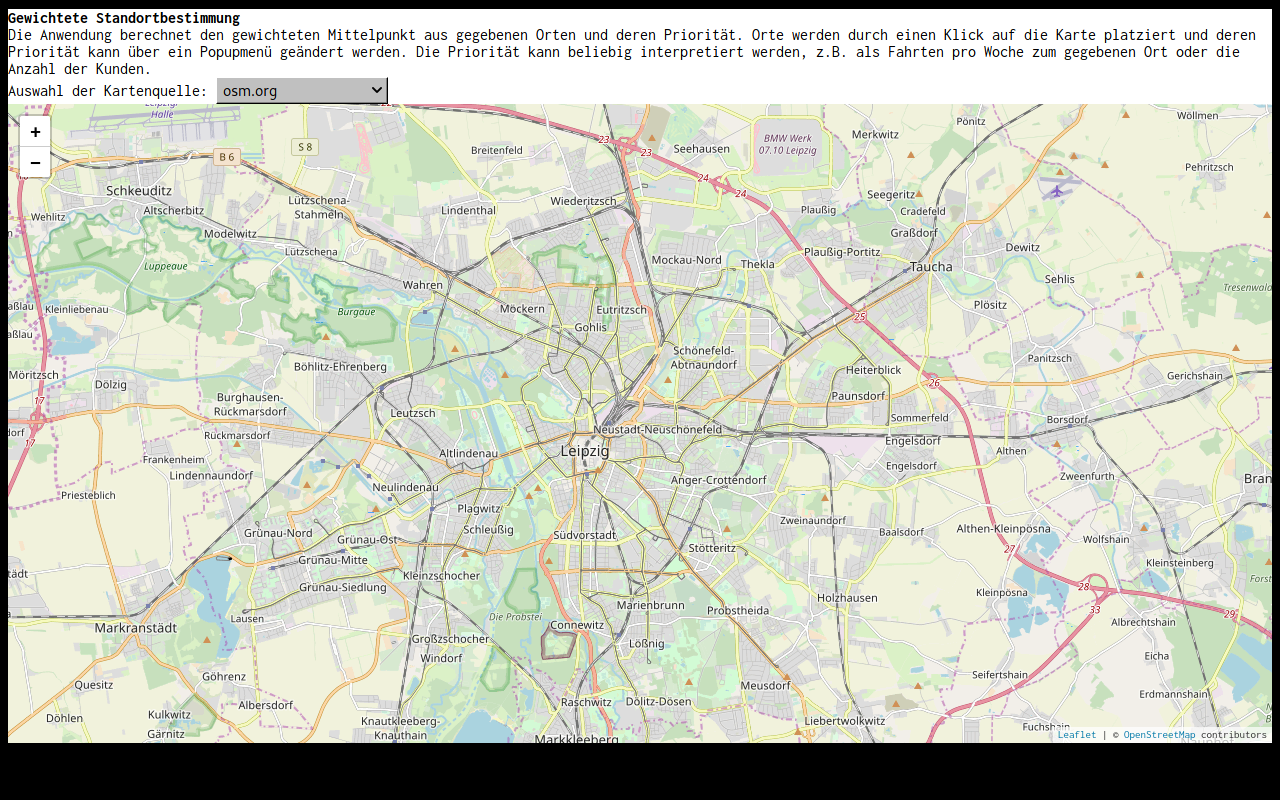
\includegraphics[width=\linewidth]{bell1_1.png}
\caption{Screenshot von der Anwendung}
\end{figure}\\
Auf dieser Karte können nun Orte angeklickt werden, woraufhin ein Marker an der entsprechenden Position gesetzt wird. Auch wird direkt ein Mittelpunkt berechnet der sich aus den Standartwerten der Marker berechnen lässt.\\
\begin{figure}[h]
\includegraphics[width=\linewidth]{bell2_1.png}
\caption{Screenshot der Anwendung mit gesetzten Markern}
\end{figure}
\\\\\\\\
Um die Priorität eines Markers zu ändern muss man diesen anklicken und dort die Priorität im Eingabefeld ändern. Auch kann man in dem Popup einen Knopf zum Entfernen des Markers drücken, falls man ihn nicht mehr braucht.\\
\begin{figure}[h]
\includegraphics[width=\linewidth]{bell3_1.png}\caption{Screenshot von Anwendung mit Marker Popup}
\end{figure}
\chapter{Diskussion}
\section{Auswertung}
Die Anwendung ist vor allem für Personen/Dienstleister geeignet, die keine besonderen Ansprüche an den Standort haben.
Vorallem Wohnvorlieben wie das Leben auf dem Land oder in der Nähe der Familie werden nicht beachtet, da dies sich nicht mit kurzen Fahrtwegen deckt.
Auch für Pendler ist diese Anwendung uninteressant, da bei diesen ihr Arbeitsort als neuer Wohnsitz vorgeschlagen wird.
Interessanter ist die Anwendung für Personen die noch bei ihren Eltern oder in einer WG wohnen, die einen Umzug planen und bereits eine feste Arbeitsstelle haben. 
\section{Ausblick}
Momentan berechnet die Anwendung die Entfernungen nur per Luftlinie und lässt Straßen und natürliche Hindernisse, wie zum Beispiel Gewässer und Wälder, außer Acht.
Somit besteht noch viel Spielraum für die Erweiterung der Anwendung, zum Beispiel Integration von einem Wegfindealgorithmus, einer veränderten Distanzrechnung(beispielsweise über die gebrauchte Zeit, ...).
Die Integration von Mietpreisen könnte auch bei der Entscheidung über den Standort helfen.
Auch die Speicherung der durch den Nutzer eingegebenen Daten in Cookies oder auf dem Server würde die Nutzerfreundlichkeit erhöhen. Oder man entwickelt eine Anwendung für Smartphones, die die Standortdaten über einen gewissen Zeitraum sammelt und diese Daten dann verarbeitet.
\bibliographystyle{abbrvdin}
\bibliography{bell}
\listoffigures
\end{document}